\chapter{Rb magnetometer characterization at UW\label{ch:characterization}}

\section{Operation modes}

 In order to determine the maximum sensitivity,an magnetometer can be operated in different mode.An atomic
magnetometer is capable of magnetic field detection in any available operation modes. Most of them found its application during the time this Master's thesis was prepared.Although main focus of this work was to study magnetometer performance in Free Induction Decay (FID) mode.
 \subsection{Forced Oscillation Mode(need to edit)}

 In this force oscillation measurement scheme we modulate the drive frequency of amplitude modulated light and  observe the magnetometer response using a lock-in amplifier.A resonance scan using lock-in amplifier can be done by demodulating the signal at the drive frequency which are act as reference frequency.For this force oscillation scan a frequency range and frequency increments are entered into the DAQ software. Via a
GPIB connection, a function generator is set to the appropriate frequencies, driving
the pump modulation of the magnetometer. The frequencies are taken by the lock-in
amplifier as a reference signal as well as the differential output of the polarimeter board
which is demodulated at the reference frequency. The resulting X and Y outputs are sent to the DAQ program, running on a computer via GPIB. 
\begin{figure}[h]
\centering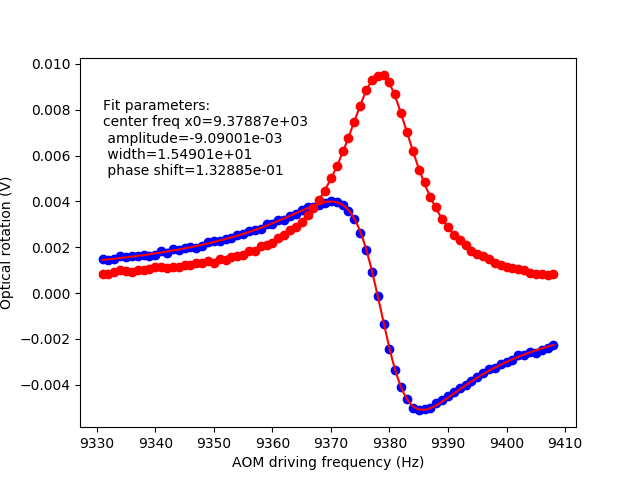
\includegraphics[width=0.4\linewidth]{figures/FM_NMOR}
\caption{Optical rotation vs. forced oscillation frequency}
\end{figure}
The quadrature components arise because exactly on resonance, the aligned atoms produce maximum optical rotation when the alignment axis is at an angle of $ \pi/4$   to the direction of the light polarization.  
The probe beam then analyzed by photodiode whose output was connected to a digital-signal-processing lock-in amplifier.The lock-in is connected to a computer via GPIB. The DAQ computer saves the lock-in data in  a Python program where the data can be analyzed. The idea of the fitting algorithm is to generate a concatenated function, having the absorptive part as the first part and the dispersive as the second (directly connected to each other). The corresponding frequency values are simply the frequency scan range for the absorptive part while the frequency increments are added to the maximum frequency point of the absorptive in order to obtain the frequency parts for the dispersive curve. This results in
the overall data for the frequency, which is inserted into the fitting function.\\
The function of absorptive part can be expressed as:
\begin{equation}
\phi_y= \frac{A_0 (X-X_0 )\omega_0}{2(X-X_0 )^2+(\omega_0^2)/4}\cos\theta-\frac{\omega_0^2A_0}{(X-X_0 )^2+(\omega_0^2/4)}\sin\theta
\end{equation}
while the dispersive part of complex lorentzian is given by 
\begin{equation}
\phi_x= \frac{A_0 (X-X_0 )\omega_0}{2(X-X_0 )^2+(\omega_0^2)/4}\sin\theta+\frac{\omega_0^2A_0}{(X-X_0 )^2+(\omega_0^2/4)}\cos\theta
\end{equation}
In this conjunction, $A_0$ represents the maximum of the purely absorptive curve, $\omega_0$ the width
of resonance (FWHM) and $x_0$ the center resonance frequency. Furthermore, x represents
the frequency values.
The overall fitting function in order to really fit a complex lorentzian is given by (the
phases in R(x) and D(x) are not considered in the following equations, since they are varied
(sin/cos)).\\


\begin{equation}
F = R(x)^{'}\theta(x \leq f_{max}) + D(x-f_{max})^{'}\theta(x > f_{max})
\end{equation}
Where 
\begin{equation}
R(x)^{'}=R(x) . \cos(\phi_0) + D(x) .\sin(\phi_0)
\end{equation}\\
and
\begin{equation}
R(x)^{'}=D(x) . \cos(\phi_0) - R(x) .\sin(\phi_0)
\end{equation}

Here, $\phi_{0} $ represents the phase shift between the absorptive and dispersive parts. This phase shift$\phi_{0}$ appears due to the wrong settings of lock-in amplifier.The actual fitting function in equation 4.3 includes a case
structure, as it is given by the Heaviside-like function $\phi(x)$. If $ (x \leq f_{max}) $ ,$\phi(x)$ becomes zero,
if $(x > f_{max})$, it is equal to one. The initial guesses for the least-square parameters are given
as:\\
\begin{itemize}
\item
Amplitude $A_0$: In order to get guess amplitude, Averaging the maximum of the absorptive and dispersive curve is done.
\item
Width $\omega_0$: A width of the resonance curve of 15 Hz is assumed.
value.
\item
Center frequency $x_0$: The maximum frequency value of the
absorptive curve is considered as a guess for the center frequency.
\item
Phase $\phi_0$: In order to get a guess for the phase, $ R =\sqrt (
X^2 + Y ^2)$ is calculated for each
X and Y data pair. The corresponding X and Y data pair which gives the maximum
R value is taken and the phase guess $\phi _0$  is calculated by $\phi _0 = arctan(Y_{max}=X_{max})$.
\end{itemize}
Advantages: In the force oscillation scan technique entire resonance curve is scanned which allow us to see if there is a pure resonance or the real resonance curve get destroyed by any other external influences. By mapping out the entire resonance curve, we can easily debug the problem because in this process we can repeatedly adjust the power of the pump and probe beam immediately after each scan. Since the output signal of the balanced photodiode is demodulated stepwise by the lock-in amplifier at the modulation frequency at each increment, small amounts of noise induce in this process which is the most advantageous point of this field measurement technique. \\
Disadvantages: The force oscillation scan is a quite slow process which is the main drawback of this measurement scheme.
For a scan range of some hundred Hz usually takes a few minutes with  waiting time of couple second. As a result the force oscillation scans are not directly sensitive to magnetic field drifts, occurring at time intervals which are shorter than the actual scan. Field drifts would cause a degradation of the precision of a swept oscillation scan.
\subsection{Self oscillation mode}
In self-oscillating mode, the output signal of photodiode is  fed back to AOM for  amplitude modulation. In this case the  output signal of polarimeter is modified to act as a square wave which drives the AOM directly. After setting the phase and gain of the feedback system properly, the system start to oscillates spontaneously  at the Larmor frequency. In order to measure the oscillation frequency a frequency counter can be used in this mode. An online tracking of the oscillating signal is also possible.
 A customized circuit board, consisting of an analog voltage amplifier, a Schmitt trigger, and two metastable circuits, is used to process optical rotation \cite{PhysRevA.62.043403}.\\
Advantages: Being a quite fast process and having a high bandwidth are the main features of this self-oscillation scan. In order to get rapid update of the magnetic field the magnetometer can be operated in this mode.\\
 Disadvantages: Since feedback loop self-oscillate in the case of constructive interference, it will work only for the signal having a phase shift of integer multiple of $ 2\pi$. This additional phase shift might be resulting into slightly off-centered resonance. As a result, self-oscillation mode is more susceptible to systematic errors in field measurement.


\subsection{Free Indution Deecay(FID) }
\bigskip
\begin{itemize}
\item The magnetometer can also
be run in free induction decay mode,where Rb atoms inside the cell is excited once and afterwards the decaying processes of the excited atoms is observed. A function generator is used to delivered the pump pulses which are necessary for pumping during a FID measurement. The output frequency of the function generator is set to the resonance frequency
\item Pumping is done for a very short time interval and the coherence decay takes place fast. The pumping process is instantaneously stopped by AOM (by applying a digital TTL signal an acousto-optic modulator can be used to shutter a laser beam on and off), which can also be used to trigger the  data acquisition (DAQ). The change in the optical rotation of probe beam is measured by balanced  photodiode and the outpu signal of the photodiode is then fed into the lock-in amplifier.
\item The reference signal on the lock-in amplifier has further to be set slightly off resonance ($\sim 100 Hz$) in internal frequency mode in order to properly record the FID.
The X and Y channels output of the lock-in amplifier are further transfered to a Tektronix oscilloscope.An python script is used to transfer the data presented on the oscilloscope screen to computer for further analysis. The entire process of pumpimg and probing during a measurement cycle in FID mode  has shown in Figure 4.2. Rb atoms are pumped using amplitude modulated laser beam for 0.1 sec and then observed the spontaneous decay of excited atoms for another 0.2 sec while the pump beam was off. \\
Table 4.1 shows the function generator and lock-in amplifier settings for FID measurement.
\begin{table}[h]
\centering
\begin{tabular}{|l |l|}
\hline

\textbf{ SETTING}    & \textbf{VALUE} \\
\hline
Function generator &   \\
\hline
Frequency & 9.4kHz   \\

Waveform    &  Square  \\

Amplitude   &  $1V_{pp}$  \\
Offset  &       500 mV  \\
Phase       &    $0\degree$ \\
Trigger     &   Manual  \\
Burst       &    1000 cycle \\
Amplitude modulation & On \\
\hline
Lock-in amplifier &     \\
\hline
Lock in frequency     & 9.297 KHz \\
Time constant     &  $300\mu s$ \\
Sensitivity      &  500mV  \\
\hline
\end{tabular}
\caption{Setting for FID at $1\mu T$ field}
\end{table}
\begin{figure}[h]
\centering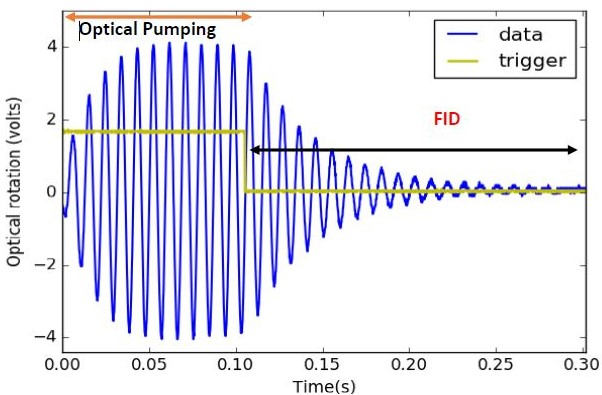
\includegraphics[width=0.55\linewidth]{figures/Capture2}
\caption{ An example of Free Induction Decay(FID) signal, when pumping the Rb atoms  was done for 0.1 sec with linearly polarized light and probing was done for 0.2 sec.The applied magnetic field during the measurement is $0.2~\mu T$. }j
\end{figure}
The signal recorded  from X channel will be a sinusoid with an exponentially damping, according to   
  \begin{equation}
                                         y(t) = y_0 + A   e^{(t-t_0)/\tau}\sin(\omega t + \phi_0)
\end{equation}  

And the signal recorded  from Y channel will be a decaying cosine wave, according to
                                       
  \begin{equation}
                                         y(t) = y_0 + A   e^{(t-t_0)/\tau}\cos(\omega t + \phi_0)
\end{equation}
where $y_0$ describes a possible offset, A is the maximum amplitude of the sinusoidal oscillation,
t the present time, $t_0$ the starting point of the measurement, $\omega$ the oscillation frequency and $\phi_0$  some possible phase shift. The data fitting procedure were done in two ways in order to study a variety of systematic effects that were encountered. One method is to take a least square fit of x and y data separately to a decaying sin and cosine wave respectively. Another way of data fitting is to fit X and Y data simultaneously. A least square-fit of the recorded data set to equation (4.6) or (4.7) gives an estimate on frequency and  therefore the magnetic field.
\begin{figure}
    \centering
 
    \begin{subfigure}[b]{0.45\textwidth}
        \centering
        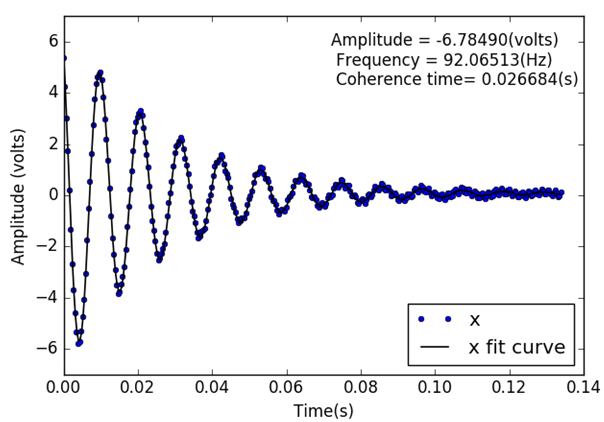
\includegraphics[width=\textwidth]{figures/fid_x_fit}
        \caption{}
        \label{fig:three sin x}
    \end{subfigure}
    \hfill
    \begin{subfigure}[b]{0.45\textwidth}
        \centering
        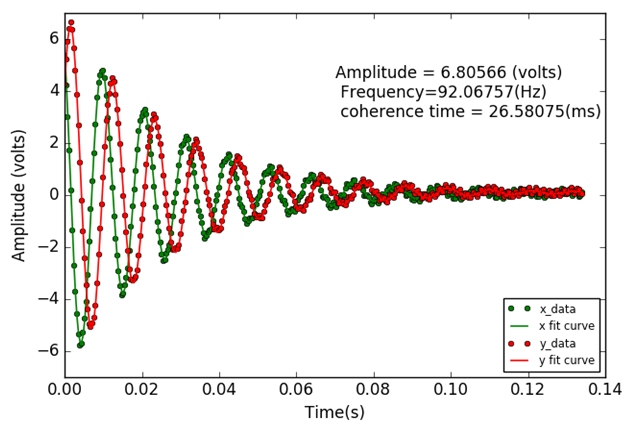
\includegraphics[width=\textwidth]{figures/fid_simultaneous}
        \caption{}
        \label{fig:five over x}
    \end{subfigure}
    \caption{(a) Least square fit of X data(blue points are x data and black curve is fitted curve ) (b) Simultaneous fit of X and Y signal(green and red dots are represents x and y data respectively whereas green and red curve represents fit curves ) }
    \label{fig:three graphs}
\end{figure}

The initial guesses for the least-square parameters are given
as:
\begin{itemize}
\item
Beat frequency $\omega$: In order to guess the beat frequency, the Fast Fourier Transform (FFT) of FID signal is done.The extracted FFT frequency is used as guess frequency.
\item
Amplitude A: In order to get guess amplitude, Averaging the maximum of the X and Y data is done.
\item
Offset $\phi_0$: The mean of FID signal is calculated. This mean value is used as guess for the offset. 

\end{itemize}
The data fitting procedure provides us the actual value for those parameters. The oscillation frequency, one of the extracted fit parameters, is then is used to estimate the magnetic field according to the following equation
\begin{equation}
B= \frac{oscilation ~ frequency +~lock in~ frequency}{2\gamma}
\end{equation}
where $\gamma$ is the gyromagnetic ratio of Rb vapor. Figure 4.4 shows an example least square fit of FID signal where (a) represents only x output of lock-in amplifier and (b) represents both x and y output of lock-in.\\
Advantages: FID mode is free of probe and pump light induced light shifts because the optical pumping is done for a very short time period and the coherence decay process takes place quickly. 

Disadvantages: As a finite duty cycle is used (pump modulation only happens during a short period of time and the main idea is to watch the coherence decay, a decreasing of the maximum achievable sensitivity with this method.


\end{itemize}

\subsection{FID in tilted magnetic field}
For the nEDM experiment it is very important to do tilted field measurement in order to have better understanding of  geometric phase effects which are the leading sources for systematic uncertainties during nEDM measurement . 
Since our Rb magnetometer is a scalar magnetometer, it is not possible to measure vector field components directly.In general, when the magnetic field is along the light propagation direction, the main resonance occurs at $\Omega_m = 2\Omega_L$.This resonance appear because of the symmetry of the optically pumped state.It is found that When magnetic field direction is tilted in the plane perpendicular to the light polarization axis, resonance is observed at  $\Omega_m = 2\Omega_L$with its amplitude depending on the tilt angle.In this case, the amplitude of resonance signal decreases with increasing tilt angle . However, If we tilt the magnetic field direction towards the light polarization axis a new resonance appears at $\Omega_L$ along with the main resonance at $2\Omega_L$ if linearly polarized light is used.In this case the resonance signal contain two frequency component(Figure 4.3(a)) . The amplitude of the new resonance signal at $\Omega_L$  increases as the angle between B and the light propagation direction increases while main resonance amplitude at $2\Omega_L$  decrease with increasing tilt angle.However,when the tilt angle is larger than some certain angle the resonance amplitude measured at $\Omega_L$ also start to decrease and reaches zero when the magnetic field is directed along the y axis.   It could be possible to evaluate the magnitude of the magnetic field from the ratio of the resonance amplitudes at $\Omega_L$ and $2\Omega_L$.The same study with frequency modulated light has been reported by Pustelny et al.\cite{PhysRevA.74.063420}. In this study the NMOR Signal was observed by connecting the balanced photodiode to the oscilloscope directly. A python script is used to transfer the data presented on the oscilloscope screen to computer for further analysis. 

\begin{figure}
    \centering
 
    \begin{subfigure}[b]{0.45\textwidth}
        \centering
        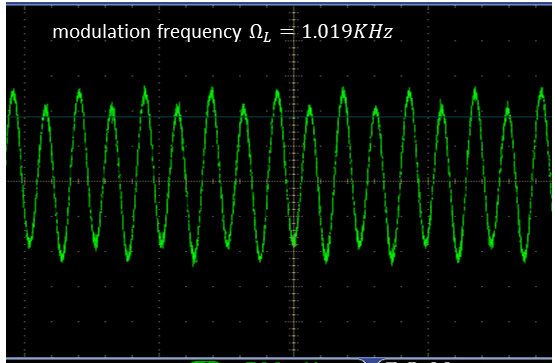
\includegraphics[width=\textwidth]{figures/transverse_field}
        \caption{}
        \label{fig:three sin x}
    \end{subfigure}
    \hfill
    \begin{subfigure}[b]{0.45\textwidth}
        \centering
        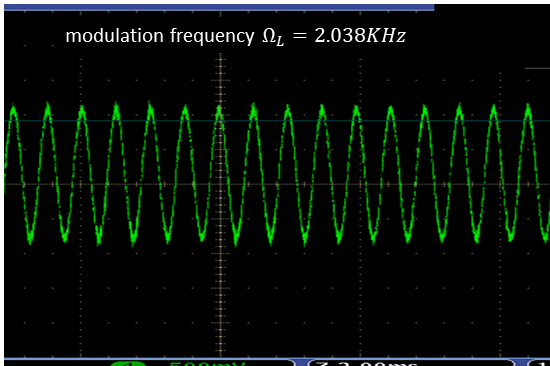
\includegraphics[width=\textwidth]{figures/transverse_field_2}
        \caption{}
        \label{fig:five over x}
    \end{subfigure}
    \caption{(a) Optical rotation as a function of time at $\Omega_L$ in the yz plane at tilt angle $15\degree$ with light propagation direction. (b) Optical rotation as a function of time at $2\Omega_L$ for same tilt angle}
    \label{fig:three graphs}
\end{figure}

